%%%%%%%%%%%%%%%%%%%%%%%%%%%%%%%%%%%%%%%%%%%%%%%%%%%%%%%%%%%%%%%%%%%%%%%%%
% This file is part of the LaTeX sources of the OMDoc 1.3 specification
% Copyright (c) 2006 Michael Kohlhase
% This work is licensed by the Creative Commons Share-Alike license
% see http://creativecommons.org/licenses/by-sa/2.5/ for details
%%%%%%%%%%%%%%%%%%%%%%%%%%%%%%%%%%%%%%%%%%%%%%%%%%%%%%%%%%%%%%%%%%%%%%%%%

\begin{tchapter}[id=math-markup]{Markup for Mathematical Knowledge}

  Mathematicians make use of various kinds of documents (e.g. e-mails, letters,
  pre-prints, journal articles, and textbooks) for communicating mathematical
  knowledge. Such documents employ specialized notational conventions and visual
  representations to convey the mathematical knowledge reliably and efficiently.  The
  respective representations are supported by pertinent   markup systems like
  {\TeX/\LaTeX}.

  Even though mathematical documents can vary greatly in their level of presentation,
  formality and rigor, there is a level of deep semantic structure that is common to all
  forms of mathematics and that must be represented to capture the essence of the
  knowledge. As John R. Pierce has written in his book on communication
  theory~\cite{Pierce:aitit80}, mathematics and its notations should not be viewed as one
  and the same thing. Mathematical ideas exist independently of the notations that
  represent them. However, the relation between meaning and notation is subtle, and part
  of the power of mathematics to describe and analyze derives from its ability to
  represent and manipulate ideas in symbolic form. The challenge in putting mathematics on
  the {\twintoo{World Wide}{Web}} is to capture both notation and content (that is,
  meaning) in such a way that documents can utilize the highly-evolved notational forms of
  written and printed mathematics, and the potential for interconnectivity in electronic
  media.

  In this chapter, we present the state of the art for representing mathematical documents
  on the web and analyze what is missing to mark up mathematical knowledge.  We posit that
  there are three levels of information in mathematical knowledge: formulae, mathematical
  statements, and the large-scale theory structure (constructing the context of
  mathematical knowledge). The first two are immediately visible in marked up mathematics,
  e.g.  textbooks, the third is largely left to an implicit meta-level of mathematical
  communication, or the organization of mathematical libraries. We will discuss these
  three levels in the next sections.

\begin{tsection}[id=math-objects]{Mathematical Objects and Formulae}

  A distinguishing feature of mathematical documents is the use of a complex and highly
  evolved system of two-dimensional symbolic notations, commonly called (mathematical)
  {\defemph{formulae}}\twin{mathematical}{formula}. Formulae serve as representations of
  {\twintoo{mathematical}{object}s}, such as {\indextoo{function}s},
  {\indextoo{group}s}, or {\twintoo{differential}{equation}s}, and
  also of statements about them, like the ``{\twintoo{Fundamental Theorem of}{Algebra}}''.

  The two best-known open markup formats for representing mathematical formulae for the
  Web are {\mathml}~\cite{CarIon:MathML03} and {\openmath}~\cite{BusCapCar:2oms04}. There
  are various other formats that are proprietary or based on specific mathematical
  software packages like {\indextoo{Wolfram Research}}'s {\mathematica}~\cite{Wolfram.02}.
  We will not concern ourselves with them, since we are only interested in open formats.
  Furthermore, we will only give a general overview for the open formats here to survey
  the state of the art, since content {\mathml} and {\openmath} are used for formula
  representation in the {\omdoc} format and thus the technical details of the two markup
  schemes are covered in more detail in the {\omdoc} specification in {\mychapref{mobj}}.
  {\myfigref{math-markup-formulae}} gives an overview over the current state of the
  standardization activities.

    \begin{myfig}{math-markup-formulae}{The Status of Markup Standardization for
        Mathematical Formulae}
      \begin{tabular}{|l|p{4cm}|p{4.4cm}|}\hline
        language & {\mathml}           & {\openmath}\\\hline\hline
        by       & W3C Math WG         & {\openmath} society\\\hline
        origin   & math for {\html}    & integration of CAS \\\hline
        coverage & content + presentation; K-14     & content; extensible \\\hline
        status   & Version 2.2e ({\rm VI} 2003) & Version 2 ({\rm VI} 2004) \\\hline
        activity & maintenance         & maintenance \\\hline
        Info     & {\small\url{http://w3c.org/Math/}} & 
                   {\small\url{http://www.openmath.org/}}    \\\hline
      \end{tabular}
    \end{myfig}

    {\openmath} was originally a development driven mainly by the Computer Algebra
    community in Europe trying to standardize the communication of mathematical objects
    between Computer Algebra Systems. The format has been discussed in a series of
    workshops and has been funded by a series of grants by the European Union. This
    process led to the {\openmath} 1 standard in June 1999 and eventually to the
    incorporation of the {\openmath} society as the institutional guardian of the
    {\openmath} standard. {\mathml} has developed out of the effort to include
    presentation primitives for mathematical notation (in {\TeX}{\index{tex@\TeX}}
    quality) into {\html}, and was the first {\xml} application\twin{XML}{application} to
    reach {\indextoo{recommendation}} status\footnote{As such, {\mathml} played a great
      role as technology driver in the development of {\xml}. This role gives {\mathml} a
      somewhat peculiar status at the W3C; it is the only ``vertical''
      (application/domain-driven) {\xml} application standardized by the W3C, which
      otherwise concentrates on ``horizontal'' (technology-driven) standards.} at the
    {\indextoo{W3C}}~\cite{IonMin:MathML99}.
    
    The competition and collaboration between these two approaches to representation of
    mathematical formulae and objects has led to a large overlap between the two developer
    communities.  {\mathml} deals principally with the {\emph{presentation}} of
    mathematical objects, while {\openmath} is solely concerned with their semantic
    meaning or {\emph{content}}.  While {\mathml} does have some limited facilities for
    dealing with content, it also allows semantic information encoded in {\openmath} to be
    embedded inside a {\mathml} structure.  Thus the two technologies may be seen as
    highly compatible\footnote{e.g. {\mathml} is the preferred presentation format for
      {\openmath} objects and {\openmath} content dictionaries are the primary
      specification language for {\mathml} semantics.} and complementary (in aim).

\begin{tsubsection}[id=math-markup:mathml]{{\mathml}}
  \begin{center}
    \fbox{\begin{minipage}{9cm} {\mathml} is an {\xml} application for describing
        mathematical {\emph{notation}} and capturing both its {\emph{structure}} and
        {\emph{content}}. The goal of {\mathml} is to enable mathematics to be served,
        received, and processed on the World Wide Web, just as {\html} has enabled this
        functionality for text.\\\strut\hfill{\emph{from the MathML2
            Recommendation}~\cite{CarIon:MathML03}}
     \end{minipage}}
 \end{center}

 To reach this goal, {\mathml} offers two sub-languages: {\pmathml} for marking up the
 two-dimensional, visual appearance of mathematical formulae, and {\cmathml} as a markup
 infrastructure for the functional structure of mathematical formulae.

 To mark up the visual appearance of formulae {\pmathml} represents mathematical formulae
 as a tree of layout primitives. For instance the expression $3\over x+2$ would be
 represented as the layout tree in {\myfigref{pmathml-tree}}. The layout primitives
 arrange ``inner boxes'' (given in black) and provide an outer box (given in gray here)
 for the next level of layout. In {\myfigref{pmathml-tree}} we see the general layout
 schemata for numbers ({\element[ns-elt=m]{mn}}), identifiers ({\element[ns-elt=m]{mi}}),
 operators ({\element[ns-elt=m]{mo}}), bracketed groups ({\element[ns-elt=m]{mfence}}),
 and fractions ({\element[ns-elt=m]{mfrac}}); others include horizontal grouping
 ({\element[ns-elt=m]{mrow}}), roots ({\element[ns-elt=m]{mroot}}), scripts
 ({\element[ns-elt=m]{msup}}, {\element[ns-elt=m]{msub}}, {\element[ns-elt=m]{msubsup}}),
 bars and arrows ({\element[ns-elt=m]{munder}}, {\element[ns-elt=m]{mover}},
 {\element[ns-elt=m]{munderover}}), and scoped {\css} styling
 ({\element[ns-elt=m]{mstyle}}). Mathematical symbols are taken from {\unicode} and
 provided with special mnemonic entities by the {\mathml} DTD, e.g. {\snippet{\&sum;}} for
 $\Sigma$.

    \begin{myfig}{pmathml-tree}{The Layout Tree for the Formula $3\over x+2$}
\begin{minipage}{2.4cm}
\begin{lstlisting}[numbers=none,frame=none]
<m:mfrac>
 <m:mn>3</m:mn>
 <m:mfenced>
   <m:mi>x</m:mi>
   <m:mo>+</m:mo>
   <m:mn>2</m:mn>
 </m:mfenced>
</m:mfrac>
\end{lstlisting}
\end{minipage}\hspace{2em}
      \begin{minipage}{8cm}
  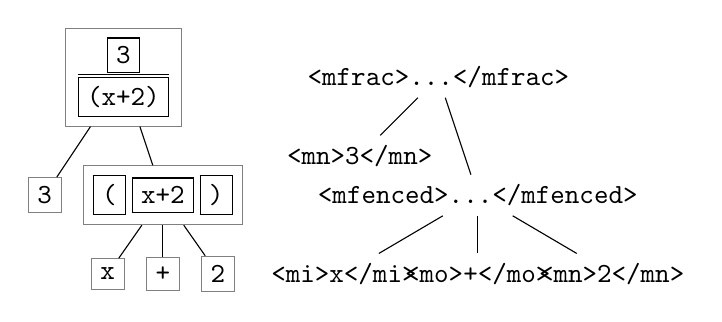
\begin{tikzpicture}
    \node[draw=gray] (frac)  at (2.5,4) {$\fbox{3}\over\fbox{(x+2)}$};
    \node[draw=gray] (3) at (1.5,2.5) {3};
    \node[draw=gray] (fence) at (3,2.5) {\fbox{(}\kern2pt\fbox{x+2}\kern2pt\fbox{)}};
    \node[draw=gray] (x) at (2.3,1.5){x};
    \node[draw=gray] (+) at (3,1.5) {+};
    \node[draw=gray] (2) at (3.7,1.5) {2};
    \draw (frac) -- (3);
    \draw (frac) -- (fence);
    \draw (fence) -- (x);
    \draw (fence) -- (+);
    \draw (fence) -- (2);

    \node (mfrac) at (6.5,4) {\tt{<mfrac>\ldots</mfrac>}};
    \node (m3) at (5.5,3) {{\tt{<mn>3</mn>}}};
    \node (mfence) at (7,2.5) {{\tt{<mfenced>\ldots</mfenced>}}};
    \node (mx) at (5.3,1.5) {{\tt{<mi>x</mi>}}};
    \node (m+) at (7,1.5) {{\tt{<mo>+</mo>}}};
    \node (m2) at (8.7,1.5)  {{\tt{<mn>2</mn>}}};
    \draw (mfrac) -- (m3);
    \draw (mfrac) -- (mfence);
    \draw (mfence) -- (mx);
    \draw (mfence) -- (m+);
    \draw (mfence) -- (m2);
  \end{tikzpicture}
\end{minipage}  
\end{myfig}

Since the aim of {\mathml} is to do most of the formatting inside the browser, where
resource considerations play a large role, it restricts itself to a fixed set of
mathematical concepts -- the {\indextoo{K-14}} fragment ({\indextoo{Kindergarten}} to
$14^{th}$ grade; i.e. undergraduate college level) of mathematics. K-14 contains a large
set of commonly used glyphs for mathematical symbols and very general and powerful
presentation primitives, similar to those that make up the lower level of {\TeX}.
However, it does not offer the programming language features of {\TeX}\footnote{{\TeX}
  contains a full, {\indextoo{Turing}}-complete -- if somewhat awkward -- programming
  language that is mainly used to write {\twintoo{style}{file}}s.  This is separated out
  by {\mathml} to the {\css} and {\xslt} style languages it inherits from {\xml}.}  for
the obvious computing resource considerations.  {\pmathml} is supported by current
versions of the browsers {\amaya}~\cite{amaya_web}, {\msie}~\cite{ie_web} (via the
{\mathplayer} plug-in~\cite{mathplayer_web}), and {\mozilla}~\cite{mozilla_web}.

  {\mathml} also offers content markup for mathematical formulae, a sub-language called
  {\defemph{{\cmathml}}} to contrast it from the {\defemph{{\pmathml}}} described
  above. Here, a mathematical formula is represented as a tree as well, but instead of
  marking up the visual appearance, we mark up the functional structure. For our example
  $3\over x+2$ we obtain the tree in {\myfigref{cmathml-tree}}, where we use @ as the
  function application operator (it interprets the first child as a function and applies
  it to the rest of the children as arguments).

\begin{myfig}{cmathml-tree}{The functional Structure of $3\over x+2$}
\begin{minipage}{3cm}
\begin{lstlisting}[numbers=none,frame=none]
<m:apply>
  <m:divides/>
  <m:cn>3</m:cn>
  <m:apply>
    <m:plus/>
    <m:ci>x</m:ci>
    <m:cn>2</m:cn>
  </m:apply>
</m:apply>
\end{lstlisting}
\end{minipage}\hspace*{3em}
\begin{minipage}{4cm}
  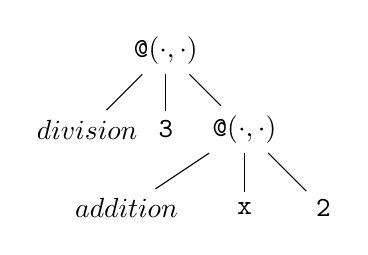
\begin{tikzpicture}
    \node (app1)  at (2.5,3.5) {$\hbox{@}(\cdot,\cdot)$};
    \node (div) at (1.5,2.5) {$division$};
    \node (3) at (2.5,2.5) {3};
    \node (app2) at (3.5,2.5) {$\hbox{@}(\cdot,\cdot)$};
    \node (plus) at (2,1.5){$addition$};
    \node (x) at (3.5,1.5) {x};
    \node (2) at (4.5,1.5) {2};
    \draw (app1) -- (div);
    \draw (app1) -- (3);
    \draw (app1) -- (app2);
    \draw (app2) -- (plus);
    \draw (app2) -- (x);
    \draw (app2) -- (2);
  \end{tikzpicture}
\end{minipage}
\end{myfig}

{\cmathml} offers around 80 specialized elements for the most common K-14 functions and
individuals. In {\myfigref{cmathml-tree}} we see function application
({\element[ns-elt=m]{apply}}), content identifiers ({\element[ns-elt=m]{ci}}), content
numbers ({\element[ns-elt=m]{cn}}) and the functions for division
({\element[ns-elt=m]{divide}}) and addition ({\element[ns-elt=m]{plus}}).

Finally, {\mathml} offers a specialized {\element[ns-elt=m]{semantics}} element that
allows to annotate {\mathml} formulae with alternative representations. This feature can
be used to provide combined content- and presentation-{\mathml} representations.
{\Myfigref{pcmml}} shows an example of this for our expression $3\over x+2$. The outermost
{\element[ns-elt=m]{semantics}} element is used for mixing presentation and content
markup. The first child of the {\element[ns-elt=m]{semantics}} element contains {\pmathml}
(this is used by the {\mathml}-aware browser), the subsequent
{\element[ns-elt=m]{annotation-xml}} element contains {\cmathml} markup for the same
formula. Corresponding sub-expressions are {\indextoo{co-reference}d} by
{\indextoo{cross-reference}s}: The presentation element carries an
{\attributeshortcomment{id}{in {\sc{MathML}}}} attribute, which serves as the target for
an {\attribute[ns-attr=xlink]{href}{in {\sc{MathML}}}} attribute in the content
markup. This technique is called {\twintoo{parallel}{markup}}, it allows to select logical
sub-expressions by selecting layout sub-schemata\twin{layout}{schema} in the browser,
e.g. for copy and paste. Note that a {\element[ns-elt=m]{semantics}} element can have more
than one {\element[ns-elt=m]{annotation-xml}} child, so that other content formats such as
{\openmath} can also be incorporated.

\begin{myfig}{pcmml}{Mixing Presentation and {\cmathml}}
  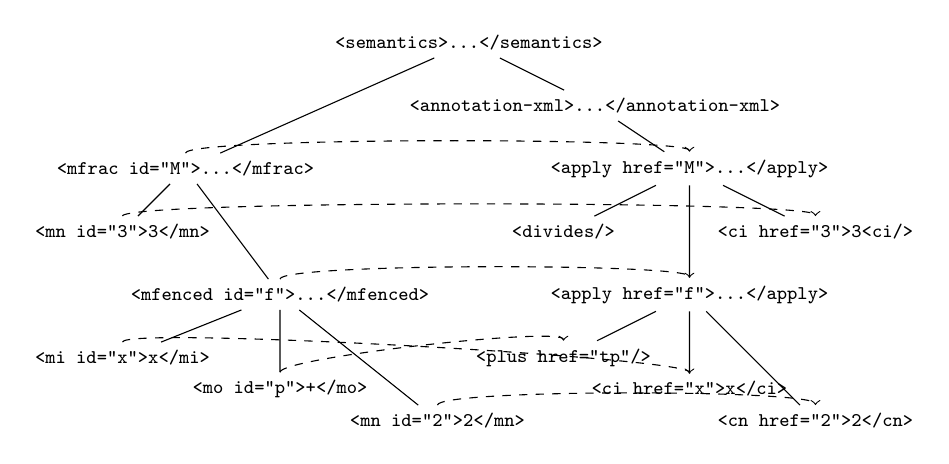
\begin{tikzpicture}[scale=.8]\scriptsize
    \tikzstyle{every node}=[font=\ttfamily]
    \node (semantics) at (6,6) {<semantics>\ldots</semantics>};
    \node (ann) at (8,5) {<annotation-xml>\ldots</annotation-xml>};
    \node (mfrac) at (1.5,4) {<mfrac id="M">\ldots</mfrac>};
    \node (m3) at (0.5,3)    {<mn id="3">3</mn>};
    \node (mfence) at (3,2) {<mfenced id="f">\ldots</mfenced>};
    \node (mx) at (0.5,1)  {<mi id="x">x</mi>};
    \node (m+) at (3,.5)     {<mo id="p">+</mo>};
    \node (m2) at (5.5,0)   {<mn id="2">2</mn>};
    \node (apply) at (9.5,4){<apply href="M">\ldots</apply>};
    \node (div) at (7.5,3)  {<divides/>};
    \node (c3) at (11.5,3)  {<ci href="3">3<ci/>};
    \node (apply2) at (9.5,2) {<apply href="f">\ldots</apply>};
    \node (plus) at (7.5,1) {<plus href="tp"/>};
    \node (cx) at (9.5,.5)  {<ci href="x">x</ci>};
    \node (c2) at (11.5,0)  {<cn href="2">2</cn>};

    \draw (semantics) -- (ann);
    \draw (semantics) -- (mfrac);
    \draw (mfrac) -- (m3);
    \draw (mfrac) -- (mfence);
    \draw (mfence) -- (mx);
    \draw (mfence) -- (m+);
    \draw (mfence) -- (m2);
    \draw (ann) -- (apply);
    \draw (apply) -- (div);
    \draw (apply) -- (apply2);
    \draw (apply) -- (c3);
    \draw (apply2) -- (plus);
    \draw (apply2) -- (cx);
    \draw (apply2) -- (c2);
    
    \draw[->,dashed] (mfrac) .. controls +(up:.5cm) and +(up:.5cm)  .. (apply);
    \draw[->,dashed] (m3) .. controls +(up:.5cm) and +(up:.5cm)  .. (c3);
    \draw[->,dashed] (mfence) .. controls +(up:.5cm) and +(up:.5cm)  .. (apply2);
    \draw[->,dashed] (m+) .. controls +(up:.5cm) and +(up:.5cm)  .. (plus);
    \draw[->,dashed] (mx) .. controls +(up:.5cm) and +(up:.5cm)  .. (cx);
    \draw[->,dashed] (m2) .. controls +(up:.5cm) and +(up:.5cm)  .. (c2);
  \end{tikzpicture}
\end{myfig}
\end{tsubsection}

\begin{tsubsection}[id=math-markup:openmath]{\openmath}
  \begin{center}
    \fbox{\begin{minipage}{9cm} [\ldots]
        {\openmath}: a standard for the representation and
        communication of mathematical objects. [\ldots]\\
        {\openmath} allows the {\emph{meaning}} of an object to be encoded rather than
        just a visual representation.  It is designed to allow the free exchange of
        mathematical objects between software systems and human beings.  On the worldwide
        web it is designed to allow mathematical expressions embedded in web pages to be
        manipulated and computed with in a meaningful and correct way.  It is designed to
        be machine-generatable and machine-readable, rather than written by
        hand.\\\strut\hfill{\emph{from the {\openmath}2 Standard}~\cite{BusCapCar:2oms04}}
      \end{minipage}}
  \end{center}

  Driven by the intention of representing the {\emph{meaning}} of mathematical objects
  expressed in the quote above, the {\openmath} format is not primarily an {\xml}
  application. Rather, {\openmath} defines an abstract (mathematical) object model for
  mathematical objects and specifies an {\xml} encoding (and a binary\footnote{The binary
    encoding allows to optimize encoding size and (more importantly) parsing time for
    large {\openmath} objects. The binary encoding for {\openmath} objects will not play a
    role for the {\omdoc} format, so we will not pursue this here.}  encoding) for
  that\footnote{The {\mathml} specification is very vague on what the meaning of
    {\cmathml} fragments might be; we have to assume that its {\xml} {\twintoo{document
        object}{model}}~\cite{URL:DOM} or the or its
    {\indextoo{infoset}}~\cite{CowTob:xis04} must be.}.

  The central construct of {\openmath} is that of an {\defemph{{\openmath}
      object}}\index{object!{\sc OpenMath}}\index{OpenMath@{\sc OpenMath}! object}
  (realized by the element {\element[ns-elt=om]{OMOBJ}} in the {\xml} encoding), which has
  a tree-like representation made up of {\indextoo{application}s}
  ({\element[ns-elt=om]{OMA}}), {\indextoo{binding structure}s}
  ({\element[ns-elt=om]{OMBIND}} using {\element[ns-elt=om]{OMBVAR}} to specify the
  {\twintoo{bound}{variable}s}\footnote{Binding structures are somewhat awkwardly realized
    via the {\element[ns-elt=m]{apply}} element with an {\element[ns-elt=m]{bvar}} child
    in {\cmathml}.}), {\indextoo{variable}s} ({\element[ns-elt=om]{OMV}}), and
  {\indextoo{symbol}s} ({\element[ns-elt=om]{OMS}}). 

  The handling of symbols --- which are used to represent the multitude of mathematical
  domain constants --- is maybe the largest difference between {\openmath} and {\cmathml}.
  Instead of providing elements for all K-14 concepts, the {\openmath} standard adds an
  extension mechanism for mathematical concepts, the {\defemph{content
      dictionaries}}\twin{content}{dictionary}.  These are {\indextoo{machine-readable}}
  documents that define the meaning of mathematical concepts expressed by {\openmath}
  symbols.  Just like the library mechanism of the {\atwintoo{C}{programming}{language}},
  they allow {\openmath} to externalize the definition of extended language concepts. As a
  consequence, {\indextoo{K-14}} need not be part of the {\openmath} language, but can be
  defined in a set of content dictionaries (see~\cite{URL:omcd-core}).

  The {\element[ns-elt=om]{OMS}} element carries the attributes {\attribute{cd}{OMS}} and
  {\attribute{name}{OMS}}.  The {\attribute{name}{OMS}} attribute gives the name of the
  symbol, the {\attribute{cd}{OMS}} attribute specifies the {\indextoo{content
      dictionary}}. As variables do not carry a meaning independent of their local
  content, {\element[ns-elt=om]{OMV}} only carries a {\attribute{name}{OMV}}
  attribute. See {\mylstref{om-comm}} for an example that uses most of the elements.

\begin{lstlisting}[label=lst:om-comm,
    caption={{\openmath} Representation of $\allcdot{a,b}{a+b=b+a}$},
    language=OpenMath,
    index={OMOBJ,OMBIND,OMS,OMBVAR,OMV,OMATTR,OMATP}]
<OMOBJ xmlns="http://www.openmath.org/OpenMath">                            
  <OMBIND cdbase="http://www.openmath.org/cd">                          
    <OMS cd="quant1" name="forall"/> 
    <OMBVAR><OMV name="a"/><OMV name="b"/></OMBVAR>                        
    <OMA><OMS cd="relation" name="eq"/> 
      <OMA><OMS cd="arith1" name="plus"/>
        <OMV name="a"/>               
        <OMV name="b"/>               
      </OMA>                         
      <OMA><OMS cd="arith1" name="plus"/>
        <OMV name="b"/>               
        <OMV name="a"/>               
      </OMA>      
    </OMA>                           
  </OMBIND>                         
</OMOBJ>
\end{lstlisting}
  {\Mylstref{om-comm}} shows the {\xml} encoding of the law of commutativity for addition
  (the formula $\allcdot{a,b}{a+b=b+a}$) in {\openmath}. Note that as we have discussed
  above, this representation is not self-contained but relies on the availability of
  content dictionaries\index{content dictionary} {\snippet{quant1}},
  {\snippet{relation1}}, and {\snippet{arith1}}. Note that in this example they can be
  accessed via the URL specified in the {\attribute[ns-elt=om]{cdbase}{OMOBJ}} attribute,
  but in general, the content dictionaries are only used for {\emph{identification of
      symbol}s}. In particular, in the classical {\openmath} model, content dictionaries
  are only viewed as a resource for system developers, who use them as a reference decide
  which symbol to use in an export/import facility for a {\twintoo{computer
      algebra}{system}}. In the communication between mathematical software systems, they
  are no longer needed: If two systems agree on a set of content dictionaries, then they
  agree on the meaning of all {\openmath} objects that can be constructed using their
  symbols (the meaning of applications and bindings is known from the folklore).

  The content dictionary architecture is the greatest strength of the {\openmath}
  format. It establishes an object model and {\xml} encoding based on what we call
  ``\twintoo{semantics}{by pointing}''. Two {\openmath} objects have the same meaning in
  this model, iff they have the same structure and all symbols point to the same content
  dictionaries\footnote{Note that we can interpret the {\cmathml} model as a ``semantics
    by pointing'' model as well. Only that here the K-14 elements do not point to
    machine-readable content dictionaries, but at the (human-readable) {\mathml}
    specification, which specifies their meaning.}.

  In the standard encoding of {\openmath} content dictionary, the meaning of a symbol is
  specified by a set of
  \begin{description}
  \item[{\bf{``formal mathematical properties\atwin{formal}{mathematical}{property}''}}]
    The {\element[ns-elt=omcd]{FMP}} element contains an {\openmath} object that expresses
    the desired property.
  \item[{\bf{``commented mathematical
        properties\atwin{commented}{mathematical}{property}''}}] The
    {\element[ns-elt=omcd]{CMP}} element contains a natural language description of a
    desired property.
  \end{description}
  For instance, the specification in {\mylstref{arith1}} is part of the standard
  {\openmath} content dictionary {\snippetin{arith1.ocd}}~\cite{URL:omcd-core} for the
  elementary arithmetic operations.\footnote{The content of the
    {\element[ns-elt=omcd]{FMP}} element is actually the {\openmath} object in the
    representation in {\mylstref{om-comm}}, we have abbreviated it here in the usual
    mathematical notation, and we will keep doing this in the remaining document: wherever
    an {\xml} element in a figure contains mathematical notation, it stands for the
    corresponding {\openmath} element.}
\begin{lstlisting}[label=lst:arith1,language=omCD,mathescape,
  caption={Part of the {\sc OpenMath} Content Dictionary {\snippet{arith1}}.},
  index={CDDefinition,Name,dc:description,CMP,FMP}]
<CDDefinition>
  <Name>plus</Name> 
  <CDDescription>
    The symbol representing an n-ary commutative function plus.
  </CDDescription> 
  <CMP><xhtml:p>for all a,b | a + b = b + a</xhtml:p></CMP>
  <FMP>$\allcdot{a,b}{a+b=b+a}$</FMP> 
</CDDefinition>
\end{lstlisting}

  On the other hand, the content dictionary encoding defined in the {\openmath} standard
  (and the particular content dictionaries blessed by the {\openmath} society) are the
  greatest weakness of {\openmath}.  The represent the knowledge in a very unstructured
  way --- to name just a few problems:
  \begin{itemize}
  \item in the {\element[ns-elt=omcd]{CMP}}, we can only make use of ASCII representation
    of formulae.
  \item The relation between a particular {\element[ns-elt=omcd]{CMP}} and
    {\element[ns-elt=omcd]{FMP}} elements is unclear.
  \item For properties like the {\indextoo{distributivity}} of addition over
    multiplication it is unclear, whether we should express this in the definition of the
    symbol {\snippet{plus}} or the symbol {\snippet{times}}.
  \item Are all properties constitutive{\twin{constitutive}{property}} for the meaning of
    the symbol? Should they be verified for an implementation of a content dictionary?
  \item What is the relationship between content dictionaries? Are they
    {\indextoo{translation-equivalent}}?  Does one entail the other?
  \end{itemize}
  The {\openmath}2 standards acknowledges these problems and explicitly opens up the
  content dictionary format allowing other representations that meet certain minimal
  criteria relegating the standard encoding above to a reference implementation of the
  minimal model.

  We will analyze the questions raised above from a general standpoint when discussing the
  remaining two levels of mathematical knowledge. This analysis constitutes the basic
  intuitions for the {\omdoc} format.
\end{tsubsection}
\end{tsection}

\begin{tsection}[id=meta-math]{Mathematical Texts and Statements}

  The mathematical markup languages {\openmath} and {\mathml} we have discussed in the
  last section have dealt with mathematical objects and formulae. The formats either
  specify the semantics of the mathematical object involved in the standards document
  itself ({\mathml}) or in a fixed set of generally agreed-upon documents ({\openmath}
  content dictionaries\index{content dictionary}). In both cases, the mathematical
  knowledge involved is relatively fixed. Even in the case of {\openmath}, which has an
  extensible library mechanism, the content dictionaries are not in themselves objects of
  communication (they are mainly background reference for the implementation of
  {\openmath} interfaces).

  For the communication among mathematicians (rather than computation systems) this level
  of support is insufficient, because the mathematical knowledge expressed in definitions,
  theorems (stating properties of defined objects), their proofs, and even whole
  mathematical theories is the primary focus of mathematical communication. For content
  markup of mathematical knowledge, we have to turn implicit or presentational structuring
  devices in mathematical documents\twin{document}{mathematical} into explicit ones. For
  instance, {\twindef{mathematical}{statement}s} like the ones in the document fragment in
  {\myfigref{fragment}} are delimited by keywords (e.g. {\bf{Definition}}, {\bf{Lemma}}
  and {\boexchen}) or by changes in text font.

\begin{myfig}{fragment}{A Fragment of a Traditional Mathematical Document}
  \fbox{\begin{minipage}{10cm}
      {\bf Definition 3.2.5} (Monoid)\\
    A monoid is a semigroup $S=(G,\circ)$ with an element $e\in G$, 
    such that $e\circ x=x$ for all $x\in G$. $e$ is called a left 
    unit of $S$.\\[1ex]
    
    {\bf Lemma 3.2.6}\\
    {\emph{A monoid has at most one left unit.}}\\
    {\bf Proof}: We assume that there is another left unit $f$ \ldots\\
    This contradicts our assumption, so we have proven the claim.\hfill\kasten
  \end{minipage}}
\end{myfig}
Of course, the content of a mathematical statement, e.g. the statement of an assertion
that ``addition is commutative'' can be expressed by a {\cmathml} or {\openmath} formula
like the one in {\mylstref{om-comm}}, but the information that this formula is a theorem
that has a proof, cannot be directly expressed without extending the formalism. Even
formalizations of mathematics like Russell and Whitehead's famous ``Principia
Mathematica''~\cite{WhiRus:pm10} treat this information on the meta-level. If we are
willing to extend the mathematical formalism to include primitives for such information,
we arrive at formalisms called {\twindef{logical}{framework}s} (see~\cite{Pfenning:lf01}
for an overview), where they are treated as the primary objects of study. The most
prevalent approach here uses the ``{\twintoo{formulae as}{types}}'' idea that delegates
{\twintoo{mathematical}{formula}e} to the status of types. Logical frameworks capture
{\twintoo{mathematical}{statement}s} in formulae and as such can be expressed in
{\cmathml} or {\openmath}.  However, this approach relies on full formalization of the
mathematical content, and cannot be directly used to capture mathematical practice. In
particular, the gap between formal mathematics and informal (but rigorous) treatments of
mathematics that rely on natural language as we find them in textbooks and journal
articles is wide.  The formalization process is so tedious, that it is seldom executed in
practice (the ``Principia Mathematica'' and the {\mizar} mathematical
library~\cite{MizarKB} are solitary examples).
\end{tsection}

\begin{tsection}[id=meta-theories]{Large-Scale Structure and Context in Mathematics}

  The large-scale structure of mathematical knowledge is much less apparent than that for
  formulae and even statements. Experienced mathematicians are nonetheless aware of it,
  and use it for navigating the vast space of mathematical knowledge and to anchor their
  communication. 

  Much of this structure can be found in networks of {\defemph{ mathematical
      theories}\twin{mathematical}{theory}}: groups of mathematical statements, e.g. those
  in a \indextoo{monograph} ``Introduction to Group Theory'' or a {\indextoo{chapter}} or
  {\indextoo{section}} in a {\indextoo{textbook}}. The relations among such theories are
  described in the text, sometimes supported by mathematical statements called
  {\twintoo{representation}{theorem}s}. We can observe that mathematical texts can only be
  understood with respect to a particular mathematical context given by a theory which the
  reader can usually infer from the document. The context can be stated explicitly
  (e.g. by the title of a book) or implicitly (e.g. by the fact that the e-mail comes from
  a person that we know works on finite groups, and that she is talking about math).

  If we make the structure of the context as explicit as the structure of the mathematical
  objects (we will speak of {\twindef{context}{markup}}), then mathematical software
  systems will be able to provide novel services that rely on this structure. We contend
  that without an explicit representation of context structure, tasks like semantics-based
  searching and navigation or object classification can only be performed by human
  mathematicians that can understand the implicitly given structure.

Mathematical theories {\twin{mathematical}{theory}} have been studied by mathematicians
and logicians in the search of a rigorous foundation for mathematical practice. They have
been formalized as collections of {\twintoo{symbol}{declaration}s} --- giving names to
mathematical objects that are particular to the theory --- and logical formulae, which
state the laws governing the properties of the theory. A key research question was to
determine conditions for the consistency of mathematical theories. In inconsistent
theories all statements are vacuously valid\footnote{A statement is valid in a theory, iff
  it is true for all models of the theory. If there are none, it is vacuously valid.}, and
therefore only consistent theories make interesting statements about mathematical objects.

It is one of the critical observations of meta-mathematics that theories can be extended
without endangering consistency, if the added formulae can be proven from the formulae
already in the theory (such formulae are called {\indextoo{theorem}s}). As a consequence,
consistency of a theory can be determined by examining the {\defin{axiom}s} (formulae
without a proof) alone. Thus the role of proofs is twofold, they allow to push back the
assumptions about the world to simpler and simpler axioms, and they allow to test the
model by deriving consequences of these basic assumptions that can be tested against the
data.
  
  A second important observation is that new symbols together with axioms defining their
  properties can be added to a theory without endangering consistency, if they are of a
  certain restricted syntactical form. These {\twindef{definitional}{form}s} mirror the
  various types of mathematical {\defin{definition}s} (e.g. equational, recursive,
  implicit definitions).  This leads to the ``{\emph{\atwintoo{principle
        of}{conservative}{extension}}}'', which states that conservative extensions to
  theories (by {\indextoo{theorem}s} and {\indextoo{definition}s}) are safe for
  mathematical theories, and that possible sources for inconsistencies\index{inconsistent}
  can be narrowed down to small sets of axioms.

  Even though all of this has theoretically been known to (meta)-mathema\-ticians for
  almost a century, it has only been an explicit object of formal study and exploited by
  mathematical software systems in the last decades. Much of the meta-mathematics has been
  formally studied in the context of proof development systems like
  {\automath}~\cite{Bruijn80} {\nuprl}~\cite{Constable86}, {\hol}~\cite{GoMe93},
  {\mizar}~\cite{Rudnicki:aomp92} and {\OMEGA}~\cite{BenzmuellerEtAl:otama97} which
  utilize strong logical systems that allow to express both mathematical statements and
  proofs as mathematical objects.  Some systems like {\isabelle}~\cite{Paulson90} and
  {\scsys{Twelf}}~\cite{Pfenning91} even allow the specification of the logic language
  itself, in which the reasoning takes place.  Such semi-automated theorem proving systems
  have been used to formalize substantial parts of mathematics and mechanically verify
  many theorems in the respective areas. These systems usually come with a library system
  that manages and structures the body of mathematical knowledge formalized in the system
  so far.

  In software engineering, mathematical theories have been studied under the label of
  ``(algebraic) specifications\twin{algebraic}{specification}''. Theories are used to
  specify the behavior of programs and software components. Under the pressure of
  industrial applications, the concept of a theory (specification) has been elaborated
  from a practical point of view to support the structured development of specifications,
  {\twintoo{theory}{reuse}}, and modularization.  Without this additional structure, real
  world specifications become unwieldy and unmanageable in practice. Just as in the case
  of the theorem proving systems, there is a whole zoo of specification languages, most of
  them tied to particular software systems.  They differ in language primitives,
  theoretical expressivity, and the level of tool support.

  Even though there have been standardization efforts, the most recent one being the
  {\casl} standard (Common Algebraic Specification Language; see~\cite{CoFI:2004:CASL-RM}) there have
  been no efforts of developing this into a general markup language for mathematics with
  attention to web communication and standards. The {\omdoc} format attempts to provide a
  content-oriented markup scheme that supports all the aspects and structure of
  mathematical knowledge we have discussed in this section. Before we define the language
  in the next chapter, we will briefly go over the consequences of adopting a markup
  language like {\omdoc} as a standard for web-based mathematics.

\end{tsection}
\end{tchapter}

%%% Local Variables: 
%%% mode: latex
%%% TeX-master: "omdoc"
%%% End: 

% LocalWords:  tex lst pcmml mrow mo mi ci InvisibleTimes xlink href csymbol cd
% LocalWords:  om OMB OMSTR OMF OME OMATP commm quant eq arith ocd omCD mathe
% LocalWords:  mathescape ti cians mathema ticians th externalize underdefined
% LocalWords:  forall FMP CMP CDDefinition ary mathweb mathematicised omdoc nat
% LocalWords:  comm Principia defn rec xmlns AutoMath Twelf mathml xlink href dc
% LocalWords:  openmath CDDescription ns elt attr cdbase mobj WG CAS pmathml mn
% LocalWords:  mfence mfrac mroot msup msub msubsup munder munderover mstyle mx
% LocalWords:  mfenced frac cmathml cn ann tp cx infoset OMOBJ OMA OMBIND bvar
% LocalWords:  OMBVAR OMV OMATTR omcd  omcd omcd omcd omcd omcd omcd omcd omcd
